\documentclass[a4paper]{article}

\usepackage{geometry}
\usepackage{amsmath}
\usepackage{fontspec}
\usepackage{graphicx}
\usepackage{minted}

\usepackage{polyglossia}
\setmainlanguage[variant=american]{english}

\usepackage{hyperref}
\usepackage{subcaption}

\title{INF4300 -- Mandatory project -- Part 1}
\author{Bjørn Rustad}
\date{\today}

\begin{document}

\maketitle

\section{Analyzing the textures}

The textures to be analyzed are shown in Figure \ref{fig:raw_mosaic}. 

\begin{figure}
    \centering
    \begin{subfigure}[b]{0.40\textwidth}
        \centering
        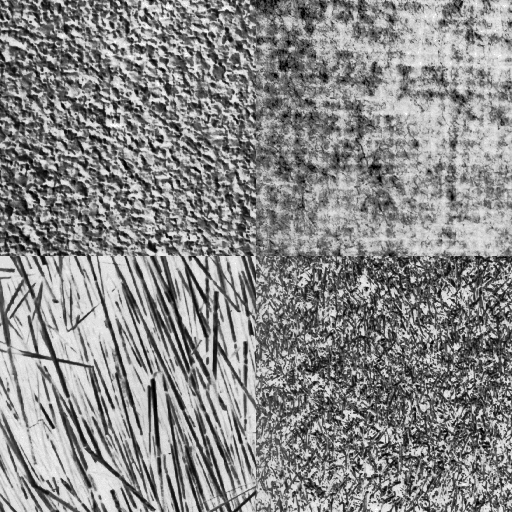
\includegraphics[width=\textwidth]{mosaic1.png}
        \caption{%
            Mosaic 1.
        }
    \end{subfigure}
    ~
    \begin{subfigure}[b]{0.40\textwidth}
        \centering
        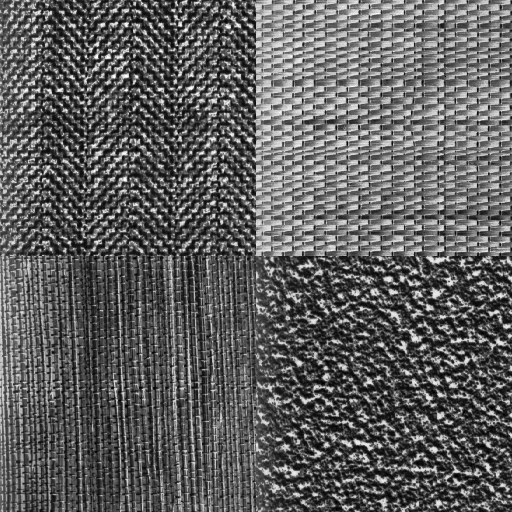
\includegraphics[width=\textwidth]{mosaic2.png}
        \caption{%
            Mosaic 2.
        }
    \end{subfigure}
    \caption{%
        Initial unprocessed mosaic images.
    }
    \label{fig:raw_mosaic}
\end{figure}

\subsection{Mosaic 1}

We start by looking at mosaic 1, which shows in the upper left corner an
relief-like texture with high contrast, no very strong directional
dependence, and a texel size of around 20x20 pixels. In the upper left
we see a more grid-like texture, where the grid is made of hair-like
structures with varying intensity. I estimate the texel size to be in
the order of 20x20 pixels also here. In the bottom left we see a very
different texture made of “sticks” laying mostly in the same direction,
and with quite high contrast. The texel size is harder to estimate, but
it is larger than in the other textures, about 40x40. In the bottom
right we have a very fine texture with no apparent direction, a small
texel size and not as high contrast as the upper left one.

\subsection{Mosaic 2}

Now in mosaic 2 we have in the upper left a fabric-like regular
structure. The texture direction varies, but in the vertical and
horizontal direction, the texture should be pretty uniform. It has a
small texel size of about 20x20. The upper right texture is a very
homogenous braid-like texture with slightly larger texel size and a
uniform texture direction. In the bottom left we have a very dark,
homogenous, bamboo-like texture with a uniform texture direction and a
texel size of about 20x20. Finally, in the bottom right we have a
homogenous but irregular texture of high contrast and no direction. It
also has a texel size of about 20x20.

\section{Visualizing the GLCM matrices}

Before analyzing the images, I perform a simple histogram equalization.
It visually seems like it enhances the contrast, and also removes some
of the spatially large variations in the background intensity. 

Then we experiment with some different values for the GLCM matrices, and
visualize them for each of the different eight textures. Most of their
textures seem to have most of their content in black and white
differences, so we start with quite a low number of levels: $G = 6$. We
use symmetric GLCM, but not isotropic, as in some matrices, we might be
interested in the directional dependence.

As mentioned in the analysis, most of the textures are either
non-directional, or are quite uniform in both the vertical and
horizontal directions, so we start by trying $(dx, dy) = \{(3, 0), (0,
3)\}$.

The results for $(dx, dy) = (3, 0)$ are shown in Figure
\ref{fig:glcm6_3_0}. We see already that the upper two, and bottom left
textures of both mosaics are kind of discernible, while the bottom right
GLCM matrix is kind of similar to the upper left matrix in both mosaics.
Looking back at the mosaics, this is not so strange, but we should be
able to separate them in some way.

\begin{figure}
    \centering
    \begin{subfigure}[b]{0.40\textwidth}
        \centering
        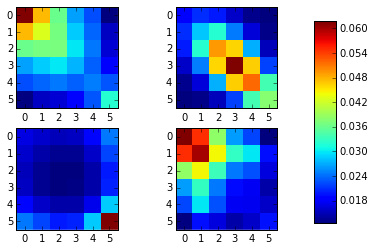
\includegraphics[width=\textwidth]{m1_3_0.png}
        \caption{%
            Mosaic 1.
        }
    \end{subfigure}
    ~
    \begin{subfigure}[b]{0.40\textwidth}
        \centering
        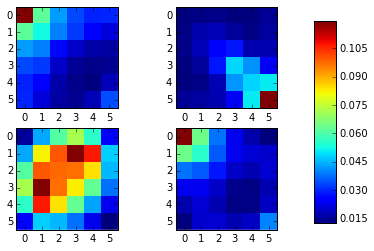
\includegraphics[width=\textwidth]{m2_3_0.png}
        \caption{%
            Mosaic 2.
        }
    \end{subfigure}
    \caption{%
        Six levels ($G = 6$), and $(dx, dy) = (3, 0)$.
    }
    \label{fig:glcm6_3_0}
\end{figure}

Although I do not expect very different results, for completeness we try
$(dx, dy) = (0, 3)$ in Figure \ref{fig:glcm6_0_3}.

\begin{figure}
    \centering
    \begin{subfigure}[b]{0.40\textwidth}
        \centering
        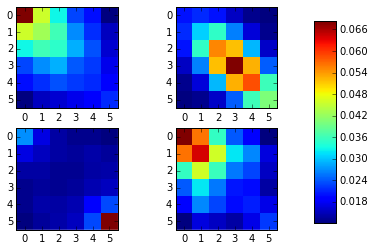
\includegraphics[width=\textwidth]{m1_0_3.png}
        \caption{%
            Mosaic 1.
        }
    \end{subfigure}
    ~
    \begin{subfigure}[b]{0.40\textwidth}
        \centering
        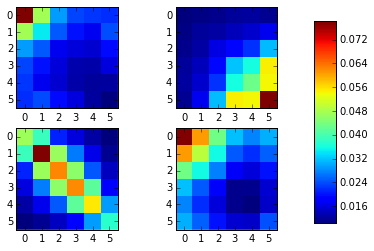
\includegraphics[width=\textwidth]{m2_0_3.png}
        \caption{%
            Mosaic 2.
        }
    \end{subfigure}
    \caption{%
        Six levels ($G = 6$), and $(dx, dy) = (0, 3)$.
    }
    \label{fig:glcm6_0_3}
\end{figure}

This is when I realize the values 0 and 3 for $dx$ and $dy$ are maybe
too small, and will be more affected by noise and small ``random''
variations than the actual texture appearance itself. Thus we try $(dx,
dy) = (10, 0)$, and to possibly increase the ``resolution'' GLCM matrix,
we increase the number of levels $G = 10$. Figure \ref{fig:glcm10_10_0}
shows the resulting matrices.

\begin{figure}
    \centering
    \begin{subfigure}[b]{0.40\textwidth}
        \centering
        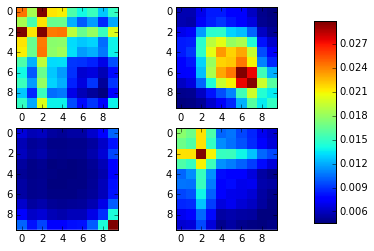
\includegraphics[width=\textwidth]{m1_10_0.png}
        \caption{%
            Mosaic 1.
        }
    \end{subfigure}
    ~
    \begin{subfigure}[b]{0.40\textwidth}
        \centering
        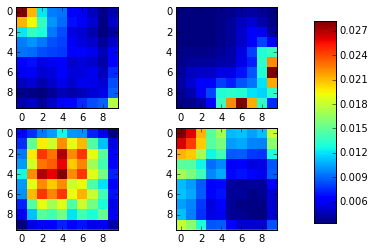
\includegraphics[width=\textwidth]{m2_10_0.png}
        \caption{%
            Mosaic 2.
        }
    \end{subfigure}
    \caption{%
        Ten levels ($G = 10$), and $(dx, dy) = (10, 0)$.
    }
    \label{fig:glcm10_10_0}
\end{figure}

As before, the top left and bottom right matrices are still a bit
similar, but now a bit more discernible if one considers the «inertia»
weighting, i.e.\ how much weight is concentrated far from the diagonal
axis.

From the three GLCM features listed in the assignment, I would think
cluster shade is the one giving the most valuable information looking at
these GLCM matrices. The cluster shade weights the matrix with a
gradient going from negative values in the upper left corner to positive
values in the lower left corner, and thus measures how the matrix is
balanced along the diagonal. Looking at the different GLCM matrices,
this could help us differentiate between all of the four textures in
each mosaic except maybe the top left from the bottom right. As the top
left square only touches the bottom right square in the middle, a
sofisticated enough segmentation step should manage to separate them
even if they have feature values in the same range.

To separate the top left from the bottom right textures, in both
mosaics, it seems like GLCM inertia would be a better feature, as the
distribution around the diagonal is a bit different, especially for the
parameters $G = 10$, $(dx, dy) = (10, 0)$ in Figure
\ref{fig:glcm10_10_0}.

\section{GLCM on local windows}

To be able to segment the textures, we calculate the GLCM matrix and
from it the GLCM features on a window that we slide over the two
mosaics. The windows are centered around a pixel, and thus we get a
feature value in each pixel position except for a border around the edge
of the image. 

We calculate the GLCM homogeneity, intertia, and cluster shade features,
and they are implemented in Appendix \ref{app:code}.

\appendix

\section{Code}
\ref{app:code}

\subsection{GLCM calculation}
\inputminted{python}{../glcm.py}

\subsection{Feature experimentation}
%\inputminted{python}{analysis.ipynb}

\end{document}

